\documentclass[]{article}
\usepackage{polski}
\usepackage[utf8]{inputenc}
\usepackage{amsmath}
\usepackage{makecell}
\usepackage[table]{xcolor}
\usepackage{graphicx}

%opening
\title{System wspomagający dystrybucję pieczywa}
\author{A. Kowalewski, M. Morusiewicz, K. Kęsik, M. Kasprzyk}

\begin{document}

\maketitle

\begin{abstract}
Niżej omawiany system może być użyteczny dla piekarni, które oprócz sklepu stacjonarnego, decydują się na dystrybucję pieczywa bezpośrednio do klienta. Dla zadanych parametrów modeli pozwala on w łatwy sposób obliczyć przychody uzyskiwane ze sprzedanego pieczywa jak i straty z powstałe przez niezaspokojenie klienta. Do tego, druga część systemu implementuje problem komiwojażera, czyli pomaga znaleźć najkrótszą trasę, jaką trzeba przejechać, aby odwiedzić wszystkich klientów.
\end{abstract}

\section{Opis matematyczny rozwiązania}

\subsection{Model doboru ilości pieczywa}

\subsubsection{Parametry sterujące modelem}

Najbardziej podstawowym zbiorem, na którym będziemy operować, jest chmura punktów - klientów, stąd też nazywać się będzie $PUNKTY$. Niech zatem

\[ p \in PUNKTY \]

gdzie $p$ jest to jeden z punktów na mapie $PUNKTY$. 

Dla każdego punktu na mapie definiujemy popyt oznaczany jako $POPYT(p)$, przy czym

\[ {\Large \forall} p \in PUNKTY \quad POPYT(p) \geq 0 \]

Oznacza to, iż w każdym obsługiwanym przez nas miejscu popyt jest nieujemny. 
	
Dla każdego punktu na mapie definiujemy cenę pieczywa $CENA(p)$, gdzie

\[ {\Large \forall} p \in PUNKTY \quad CENA(p) \geq 0 \]

Różność cen wynika z różnorodności mapy. Na pewnych obszarach wprowadzona może być promocja tudzież rabaty dla stałych klientów.
	
Dla każdego punktu na mapie możemy wyróżnić ponadto wagę niezadowolenia klienta, którą oznaczymy jako $WAGA\_NIEZADOWOLENIA(p)$, gdzie

\[ {\Large \forall} p \in PUNKTY \quad WAGA\_NIEZADOWOLENIA(p) \geq 0 \]

Niezadowolenia klienta zależy od niedoboru podaży. Wpływa to negatywnie na zyski, gdyż obniża prawdopodobieństwo kupienia pieczywa przez klienta następnym razem. Waga niezadowolenia natomiast określa to, jak uwzględniamy niezadowolenie danego klienta. Im wyższa waga, tym bardziej patrzymy na niezadowolenie w danym miejscu, a mniej na całkowity zysk ze sprzedaży.

\subsubsection{Zmienne modelu}

Dla każdego punktu mapy określamy zmienną $SPRZEDAZ$, czyli ilość bochnów sprzedanych klientom, zatem

\[ \forall p \in PUNKTY \quad SPRZEDAZ(p) \geq 0 \]

Dla każdego punktu mapy mamy także niezadowolenie klienta, o którym już wspomnieliśmy, czyli 

\[ \forall p \in PUNKTY \quad NIEZADOWOLENIE(p) \geq 0 \]

\subsubsection{Funkcja celu i ograniczenia}

Celem modelu jest maksymalizacja zysków ze sprzedaży pieczywa, a zarazem minimalizacja strat związanych z niezaspokojeniem potrzeb klienta, co symbolicznie można zapisać jako

\[
\max \left( \sum_{\forall p \in PUNKTY} SPRZEDAZ(p) \cdot CENA(p) \right)
\]

\[
\min \left( \sum_{\forall p \in PUNKTY} WAGA\_NIEZADOWOLENIA(p) \cdot NIEZADOWOLENIE(p) \right)
\]

Do opisanej funkcji celu definiujemy ponadto ograniczenie na podaż:

\[
\sum_{\forall p \in PUNKTY} SPRZEDAZ(p) = PODAZ
\]

oraz ograniczenie na popyt:

\[
\forall p \in PUNKTY \quad SPRZEDAZ(p) \leq POPYT(p)
\]

Potrzebna jest także matematyczna definicja niezadowolenia klienta. Na chwilę obecną, przyjęta została następująca prosta wersja:

\[
\forall p \in PUNKTY \quad NIEZADOWOLENIE(p) = POPYT(p) - SPRZEDAZ(p)
\]

czyli niezadowolenie rośnie wraz ze wzrostem ilości niesprzedanego pieczywa.

\subsection{Model doboru optymalnej trasy}

\subsubsection{Parametry sterujące modelem}

Tak jak w poprzednim modelu, rozpatrujemy zbiór punktów $PUNKTY$. Do tego, rozważamy parametr $DROGI$, powstający bezpośrednio z poprzedniego. Jest to zbiór wszystkich par punktów oznaczający wszystkie drogi przebiegające między punktami:

\[
DROGI = PUNKTY \times PUNKTY
\]

Na mapie punktów definiujemy także piekarnię:

\[
\exists p \in PUNKTY, \quad p = PIEKARNIA
\]

Dla każdej drogi (pary punktów) definiujemy jej długość (odległość między nimi):

\[
\forall d \in DROGI, \quad ODLEGLOSC(d) \geq 0
\]

\subsection{Zmienne modelu}

Zakładamy, iż każdą drogę używamy tylko raz (wymaga to odpowiedniej mapy):

\[
	\forall (d_1, d_2) \in DROGI, UZYCIE\_DROGI(d_1, d_2) \in \{0, 1\}
\]

Deklarujemy także zmienną pomocniczą, mówiącą o kolejności punktów wyznaczonych jako trasę:

\[
	\forall p \in PUNKTY, \quad KROK\_ODWIEDZENIA(p) \geq 0
\]

\subsubsection{Funkcja celu i ograniczenia}

Funkcja celu polega na wyznaczeniu najkrótszej trasy dla zadanej mapy:

\[
	\min \left( \sum_{(d_1, d_2) \in DROGI} ODLEGLOSCI(d_1, d_2) \cdot UZYCIE\_DROGI(d_1, d_2) \right)
\]

Potrzebne jest ponadto ograniczenie zapewniające dojechanie do każdego punktu:

\[
	\forall d_1 \in DROGI, \quad \sum_{d_2 \in DROGI} UZYCIE\_DROGI(d_1, d_2) = 1
\]

oraz zapewniające, że wyjedziemy z każdego punktu:

\[
	\forall d_2 \in DROGI, \quad \sum_{d_1 \in DROGI} UZYCIE\_DROGI(d_1, d_2) = 1
\]

Potrzebne jest też ograniczenie, by wymusić obecność tylko jednego cyklu:

\begin{align}
\forall (p_1, p_2) \in PUNKTY, &\quad KROK\_ODWIEDZENIA(p_1) - KROK\_ODWIEDZENIA(p_2) \nonumber \\&+ N \cdot UZYCIE\_DROGI(p_1, p_2) \leq N - 1 \nonumber
\end{align}

gdzie $N$ jest to łączna ilość punktów na mapie.

Ponadto ograniczenie spójności, czyli że dana droga jest użyta tylko raz:

\[
\forall (d_1, d_2) \in DROGI, \quad UZYCIE\_DROGI(d_1, d_2) + UZYCIE\_DROGI(d_2, d_1) \leq 1
\]

\section{Testy rozwiązania}

Do pierwszych testów użyliśmy bardzo prostych danych, składających się sześciu miast, oznaczanych kolejno $a,b,c,d,e,f$. Poniższa tabela przedstawia popyty i ceny występujące w każdym punkcie:

\[
\begin{array}{|c|c|c|}
	\hline
	\cellcolor{lightgray} p \in PUNKTY & \cellcolor{lightgray} POPYT(p) & \cellcolor{lightgray} CENA(p) \\ 
	\hline
	a & 200 & 1.5 \\ 
	\hline
	b & 100 & 2.5 \\ 
	\hline
	c & 300 & 3 \\ 
	\hline
	d & 400 & 2 \\ 
	\hline
	e & 50 & 5 \\ 
	\hline
	f & 1000 & 1 \\
	\hline
\end{array} 
\]

Podaż została ustawiona na wartość 800. Wagi niezadowolenia dla wszystkich punktów są jednakowe i dla różnych testów przyjmowały wartości ze zbioru $\{0.1, 1.5, 2, 3.5, 7\}$

Piekarnię ustawiliśmy w punkcie $a$, natomiast mapę dróg rozplanowaliśmy następująco:

\[
\begin{array}{|c|c|}
\hline
\cellcolor{lightgray} d \in DROGI & \cellcolor{lightgray} ODLEGLOSC(d) \\ 
\hline
a \rightarrow b & 10  \\ 
\hline
a \rightarrow c & 300  \\ 
\hline
a \rightarrow f & 25  \\
\hline
b \rightarrow c & 20  \\ 
\hline
c \rightarrow d & 15 \\ 
\hline
c \rightarrow e & 60 \\ 
\hline
c \rightarrow f & 700  \\ 
\hline
d \rightarrow e & 30  \\ 
\hline
d \rightarrow f & 150  \\ 
\hline
e \rightarrow f & 5  \\ 
\hline
\end{array} 
\]

Na rysunkach ~\ref{fig:Hf_0_1}, ~\ref{fig:Hf_1_5}, ~\ref{fig:Hf_2_0}, ~\ref{fig:Hf_3_5}, ~\ref{fig:Hf_7_0} zamieściliśmy wyniki sprzedaży w poszczególnych miastach w zależności od przyjętej wagi niezadowolenia.

\begin{figure}
	\centering
	\caption{}
	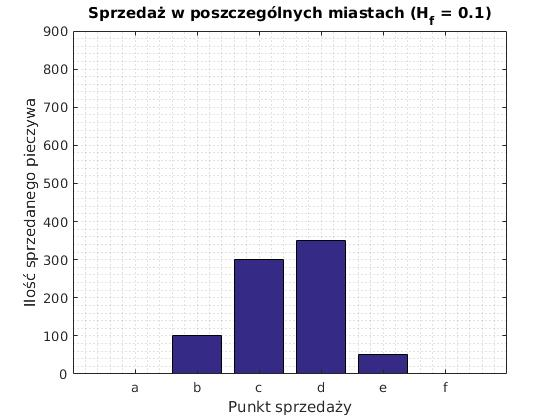
\includegraphics[width=0.7\linewidth]{Hf_0_1}
	\label{fig:Hf_0_1}
\end{figure}

\begin{figure}
	\centering
	\caption{}
	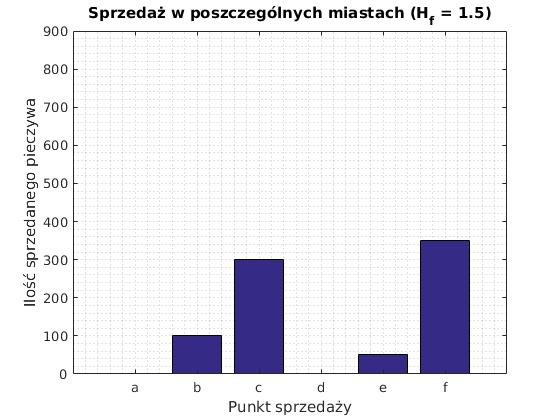
\includegraphics[width=0.7\linewidth]{Hf_1_5}
	\label{fig:Hf_1_5}
\end{figure}

\begin{figure}
	\centering
	\caption{}
	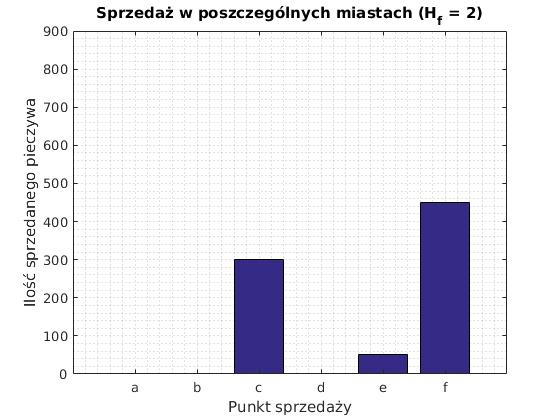
\includegraphics[width=0.7\linewidth]{Hf_2_0}
	\label{fig:Hf_2_0}
\end{figure}

\begin{figure}
	\centering
	\caption{}
	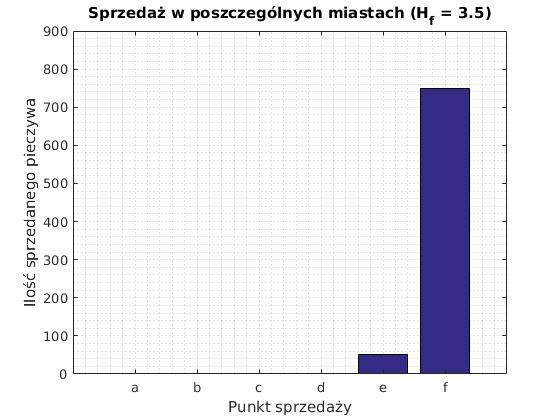
\includegraphics[width=0.7\linewidth]{Hf_3_5}
	\label{fig:Hf_3_5}
\end{figure}

\begin{figure}
	\centering
	\caption{}
	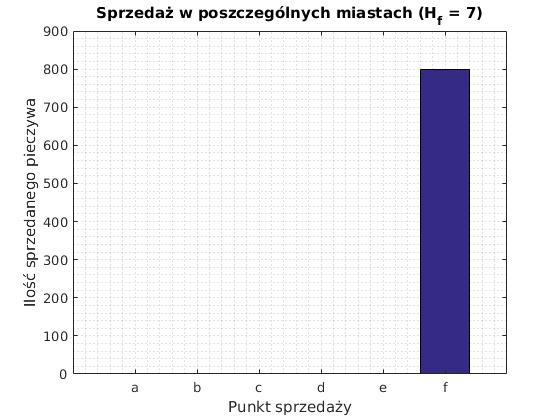
\includegraphics[width=0.7\linewidth]{Hf_7_0}
	\label{fig:Hf_7_0}
\end{figure}

Na rysunku ~\ref{fig:zysk} przedstawiliśmy zbiorczy rysunek obrazujący zysk ze sprzedaży w zależności od współczynnika wag niezadowolenia.

\begin{figure}
\centering
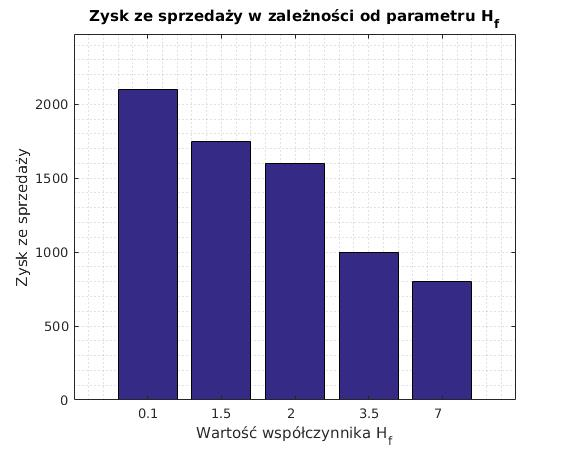
\includegraphics[width=0.7\linewidth]{zysk}
\caption{}
\label{fig:zysk}
\end{figure}

Na rysunku~\ref{fig:fcja_celu} pokazaliśmy zaś, jak zmienia się wartość funkcji celu w zależności od wag niezadowolenia.

\begin{figure}
\centering
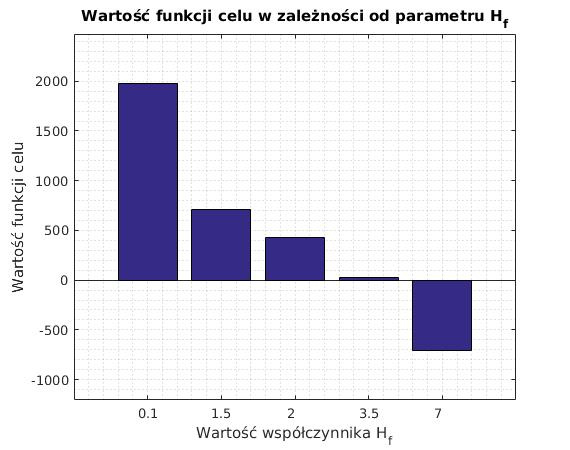
\includegraphics[width=0.7\linewidth]{fcja_celu}
\caption{}
\label{fig:fcja_celu}
\end{figure}


\end{document}
